\documentclass[../TDE1-E2.tex]{subfiles}%

\begin{document}
\section[s]"2"{Calcul d'intensité}

  \begin{center}
    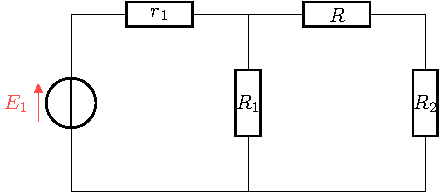
\includegraphics[scale=1]{calc_intens-plain}
  \end{center}
  \QR{%
    En utilisant les lois fondamentales dans l'ARQS
  (dites \textit{lois de Kirchhoff}), exprimer l'intensité traversant $R$ dans
  le circuit ci-contre. 
  }{%
\vspace{-15pt}
\begin{tcbraster}[raster columns=5, raster equal height=rows]
    \begin{tcn}[raster multicolumn=3](data){Schéma}
        \begin{center}
            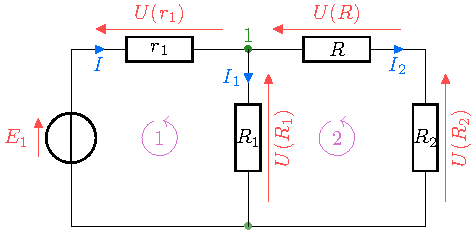
\includegraphics{calc_intens}
        \end{center}
    \end{tcn}
    \begin{tcolorbox}[blankest, raster multicolumn=2, space to=\myspace]
        \begin{tcbraster}[raster columns=1]
            \begin{tcn}[add to natural height=\myspace](ques)'r'{Résultat attendu}
                On cherche à exprimer $I_2$.
            \end{tcn}
            \begin{tcn}(tool)'r'{{LdN, LdM}}
                \begin{itemize}
                    \item $I = I_1 + I_2 \color{ForestGreen}(1)$ (LdN)~;
                    \item $I_1R_1 + Ir_1 = E_1 \color{ForestGreen}(2)$ (LdM 1)~;
                    \item $I_2(R+R_2) = I_1R_1 \color{ForestGreen}(3)$ (LdM 2).
                \end{itemize}
            \end{tcn}
        \end{tcbraster}
    \end{tcolorbox}
\end{tcbraster}
\begin{tcbraster}[raster columns=2, raster equal height=rows]
    \begin{tcn}(impo){Conseil}
        Pour les systèmes, il faut~: numéroter les équations qu'on veut
        réutiliser en premier lieu, à l'aide des $\color{ForestGreen}(1)$ par
        exemple, savoir qu'un système de 3 équations (indépendantes) à 3
        inconnues \underline{est} résolvable ensuite, et comprendre comment s'y
        prendre enfin. Cette dernière partie est bien sûr la vraie étape
        difficile et passe par la pratique, mais elle s'apprend.
    \end{tcn}
    \begin{tcn}*(rema)"lrem"'r'{Exemple}
        $I_2$ apparaît dans l'équation $\color{ForestGreen}(3)$, mais s'exprime
        en fonction de $I_1$ inconnu. On doit donc commencer par trouver une
        expression de $I_1$ utile. $I_1$ fait partie de l'équation
        $\color{ForestGreen}(2)$ qui, elle, dépend de $I$ mais en utilisant
        $\color{ForestGreen}(1)$ on peut facilement changer
        $\color{ForestGreen}(2)$ en une nouvelle équation reliant $I_1$ à $I_2$
        \underline{et qui n'est pas $\color{ForestGreen}(3)$} et qu'on
        appellera brillamment $\color{ForestGreen}(4)$. Ainsi, en réinjectant
        \textcolor{ForestGreen}{(4)} dans \textcolor{ForestGreen}{(3)}, on aura
        une expression de $I_2$ en fonction uniquement des paramètres du circuit
        ($E, R$).
    \end{tcn}
\end{tcbraster}

\begin{center}
    \begin{tcn}[sidebyside, righthand ratio=.55](appl){Application}
        Injecter \textcolor{ForestGreen}{(1)} dans \textcolor{ForestGreen}{(2)}
        donne~:
        \begin{align*}
            I_1R_1 + (I_1+I_2)r_1 &= E_1\\
            I_1(R_1+r_1) &= E_1-I_2r_1\\
            I_1 &= \frac{E_1 - I_2r_1}{R_1 + r_1} \quad \color{ForestGreen}(4)
        \end{align*}
        Ainsi, il suffit de réinjecter \textcolor{ForestGreen}{(4)} dans
        \textcolor{ForestGreen}{(3)} pour avoir~:
        \tcblower
        \begin{align*}
            I_2(R_2+R) &= \frac{E_1 - I_2r_1}{R_1 + r_1}\times R_1\\
            I_2(R_2+R)\times(R_1+r) &= (E_1-I_2r)\times R_1\\
            I_2 \left[ (R_2+R)(R_1+r_1)+r_1R_1 \right] &= E_1R_1
        \end{align*}
        et finalement
        \[\boxed{I_2 = \frac{E_1R_1}{\left[ (R_2+R)(R_1+r_1)+r_1R_1 \right]}}\]
    \end{tcn}
\end{center}
  }%
  \QR{%
      Faire de même avec un pont diviseur de courant d'une part.
  }{%
\vspace{-15pt}
\begin{tcbraster}[raster columns=2, raster equal height=rows]
    \begin{tcn}[](ques){Résultat attendu}
        On cherche à trouver $I_2$ \textit{avec un diviseur de courant}.
    \end{tcn}
    \begin{tcn}[sidebyside, righthand ratio=0.4](tool)'r'{Outil}
        \begin{center}
            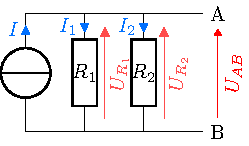
\includegraphics[]{divcour}
        \end{center}
        \tcblower
        \begin{center}
            Dans le circuit ci-contre,
            \[ I_2 = \frac{R_{\rm eq}}{R_2}I\]
        \end{center}
    \end{tcn}
\end{tcbraster}
\begin{tcn}[](data){Schéma}
    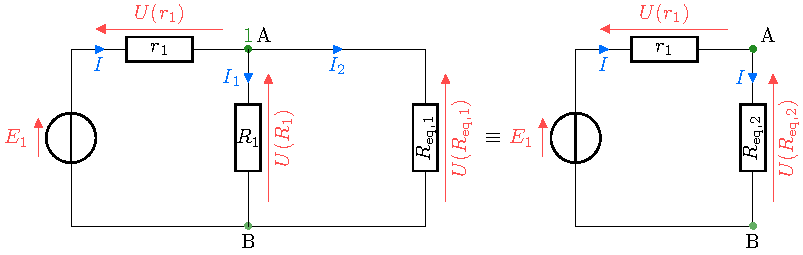
\includegraphics[width=\linewidth]{calc_intens-divcour}
\end{tcn}
\begin{tcn}[breakable, sidebyside](appl){Application}
    Sur le schéma ci-dessus, on définit
    \[ \boxed{R_{\rm eq,1} = R+R_2} \qet \boxed{R_{\rm eq,2} =
        \frac{R_1(R+R_2)}{R + R_1 + R_2}}\]
    pour appliquer la relation du pont diviseur de courant~:
    \begin{equation*}
        I_2                 = \frac{R_{\rm eq, 2}}{R_{\rm eq,1}}I
        \Leftrightarrow I_2 = \frac{R_1}{R + R_1 + R_2}I
    \end{equation*}
    \tcblower
    Avec une loi des mailles on trouve
    \begin{equation*}
        I                 = \frac{E_1}{r_1 + R_{\rm eq,2}}
        \Leftrightarrow I = \frac{E_1}{r_1 + \frac{R_1(R+R_2)}{R + R_1 + R_2}}
    \end{equation*}
    Ainsi
    \begin{gather*}
        I_2 = \frac{R_1}{\cancel{\color{orange!70}R + R_1 + R_2}}
            \frac{E_1}{r_1 \textcolor{orange!70}{(R+R_1+R_2)}
                    + \frac{R_1(R+R_2)}{\cancel{\color{orange!70}R + R_1 +
                R_2}}}\\
        \Leftrightarrow \boxed{I_2 = \frac{R_1E_1}{(R+R_1+R_2)r_1 + R_1(R+R_2)}}
    \end{gather*}
    On trouve bien le même résultat (en développant un peu).
\end{tcn}
  }%
  \QR{%
      Faire de même avec un diviseur de tension d'autre part.
  }{%
\vspace{-15pt}
\begin{tcbraster}[raster columns=2, raster equal height=rows]
    \begin{tcn}[](ques){Résultat attendu}
        On cherche à trouver $I_2$ \textit{avec un diviseur de tension}.
    \end{tcn}
    \begin{tcn}[sidebyside, righthand ratio=.4](tool)'r'{Outil}
        \begin{center}
            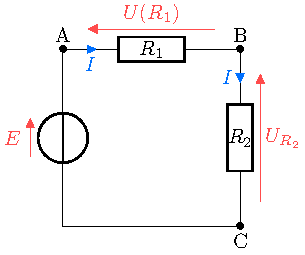
\includegraphics[width=\linewidth]{divtens-rangle}
        \end{center}
        \tcblower
        \begin{center}
            Dans le circuit ci-contre,
            \[ U_{R_2} = \frac{R_2}{R_1+R_2}E\]
        \end{center}
    \end{tcn}
\end{tcbraster}
\begin{tcn}[breakable, sidebyside](appl){Application}
    Sur le schéma ci-dessus, on définit
    \[ \boxed{R_{\rm eq,1} = R+R_2} \qet \boxed{R_{\rm eq,2} =
        \frac{R_1(R+R_2)}{R + R_1 + R_2}}\]
    pour appliquer la relation du pont diviseur de tension~:
    \begin{equation*}
        I_2(R_{\rm eq,1}) = U_{AB} =
            \boxed{U_{R_{\rm eq,2}} = \frac{R_{\rm eq,2}}{r_1 + R_{\rm eq,2}}E}
    \end{equation*}
    \tcblower
    En développant on trouve
    \begin{gather*}
        I_2\cancel{(R+R_2)} =\\
            \frac{R_1\cancel{(R+R_2)}}{\cancel{\color{orange!70}R + R_1 + R_2}}
            \frac{E}{r_1 \textcolor{orange!70}{(R+R_1+R_2)}
                    + \frac{R_1(R+R_2)}{\cancel{\color{orange!70}R + R_1 +
                R_2}}}
    \end{gather*}
    Ce qui donne bien
    \begin{equation*}
        \boxed{I_2 = \frac{R_1E}{(R+R_1+R_2)r_1 + R_1(R+R_2)}}
    \end{equation*}
\end{tcn}
  }%

\end{document}
